\documentclass[12pt]{article}

\usepackage{mathtools}
\usepackage{blindtext}

\usepackage[margin=1in]{geometry}

\newcommand*{\eu}{e}
\newcommand*{\iu}{i}

\DeclarePairedDelimiter{\bra}{\langle}{\rvert}
\DeclarePairedDelimiter{\ket}{\lvert}{\rangle}
\DeclarePairedDelimiterX{\braket}[2]{\langle}{\rangle}
  {#1\,\delimsize\vert\,\mathopen{}#2}


\usepackage[
backend=biber,
style=alphabetic,
sorting=ynt
]{biblatex}
\addbibresource{report.bib}

\usepackage[hidelinks]{hyperref}

\title{Solving Decoherence Channels on Open Quantum Systems}
\author{David Basoco \and Jack Hetherington \and Davis Rash \and Tim Ross}
\date{November 8, 2023}

\begin{document}
  \maketitle

  % TODO:
  %  - We've never cited anything. Just mention that this work is based on the
  %    specific paper in the introduction.
  %  - Add the info to the .bib file.
  %  - The paper is 1032 words. The rubric asks for 500 words.

  \section{Introduction}

  No quantum system is perfectly isolated from the environment. The case for the closed quantum systems, where the equation of motion is fully describing the state dynamics is the Schr\"{o}dinger equation. Generally, the dynamics of open quantum systems are described by a master equation, usually Lindbladian. Only under certain assumptions, known as the Born--Markov approximation, one can get an equation in this form able to describe the physical evolution of the quantum states. When these assumptions are not satisfied, we enter the non-Markovian realm. This distinction and breakdown of equations in changing scope illustrates how the open quantum systems theories are far from being completely solved.

  We will cover several test beds for experimental research into open quantum systems. These test bed classes include depolarizing and Pauli channels, Markovian reservoir engineering and amplitude damping. These experimental results demonstrate the versatile nature of quantum simulators and how they can be used for verifying and exploration into open quantum physics.

  This work is based on the article "IBM Q Experience as a versatile experimental testbedfor simulating open quantum systems" \cite{openQuantumSystems}.


  \section{Applications}

  As we continue to make quantum computers larger, we generate macro systems that begin to enter the classical realm. As these systems grow the natural decoherence of quantum phenomenon rapidly increases. This results in quantum systems that rapidly decohere in the presence of the environment or other micro states. The range is vast for this field of inquiry. From solid state physics to quantum field theory, from quantum chemistry and biology to quantum thermodynamics, numerous fields stand to benefit from understanding how macro quantum states interact and form the classical regime we interact with daily.


  \section{Depolarizing and Pauli Channels}

  The depolarizing channel was examined by first applying it on a stationary state (\( \ket{\psi_{0}} = U(\frac{\pi}{4}, \frac{\pi}{4}, 0) \ket{0} \)), with increasing values for \( p \), the probability of error. It was shown that the system was decohering into an \( I / 2 \) state as desired by plotting the real diagonal values and the real and imaginary of one of the off-diagonals. The real of the diagonal values both went to \( \frac{1}{2} \) as \( p \) increased, and both components of the off-diagonal went to \( 0 \), which shows that the state was progressing towards an \( I / 2 \) state as intended. These results are displayed in results, Fig.~\ref{fig:depolarizing_probability_state}. 

  The depolarizing channel was examined further by applying it to an oscillating circuit and time evolving that circuit with increasing decay rates. The expectation value of the \( \ket{0} \) state of the oscillating system was plotted over time. In all cases where the decay rate is greater than \( 0 \), the expectation value of \( \ket{0} \) decohered to \( \frac{1}{2} \) over time instead of continuing to oscillate, whereas the case where they decay rate was \( 0 \), the circuit continued to oscillate between \( 1 \) and \( 0 \). These results are shown in results Fig.~\ref{fig:depolarization_deay_oscillating}.

  The Pauli channel was examined by first starting a initializing a system and memory qubit in the Bell state \( \ket{\psi^{-}} \). The Pauli channel was added to the circuit affecting the system qubit. This circuit was time evolved and the rate of decoherence was effected by the values time, \( \eta \), and \( \omega \). These three values affect the probabilities of the three Pauli gates, and there are two different methods used to generate the probabilities of the gates from these parameters, the non-CP-divisible map (NCP) and the eternally non-Markovian (ENM). The work extractable was calculated from the system and memory state, and was plotted over time for each of the two methods. This gave us a similar plot to that shown in the reference material. These results are shown in results Fig.~\ref{fig:Pauli_work_extractable}.

  All figures for Depolarizing and Pauli channels were generated from runs on the IBM qasm-simulator.

  \section{Markovian Reservoir Engineering}
  We perform a simulation of the reservoir engineering circuit with \texttt{ibmq\_qasm\_simulator}. The results are shown in Fig.~\ref{fig:reservoir-engineering-simulation}. Specifically, we simulate using the environment to turn a two-qubit computational basis state into a maximally entangled state. This is called Bell-state pumping. We can see that the state is being pumped into the maximally entangled state \( \ket{\psi^{-}} \) as the fidelity of the state approaches \( 1 \) by successive \( \sigma^{z}_{1} \otimes \sigma^{z}_{2} \) and \( \sigma^{x}_{1} \otimes \sigma^{x}_{2} \) pumps.

  \section{Amplitude Damping}
  The circuit to implement the amplitude damping channel with the non-Markovianity witness as shown below. The witness is based on the behaviour of an initial maximally entangled state of qubit and auxiliary ancilla, and requires only the measurement of the expectation values of local observables.

  \begin{figure}
    \centering
    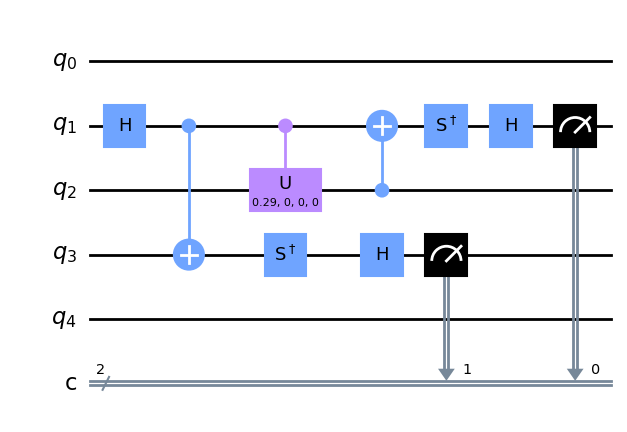
\includegraphics[width=0.7\textwidth]{images/amplitude_damping_yy_circuit.png}
    \caption{The circuit to implementing amplitude damping with the non-Markovianity witness.%
      \label{fig:amplitude_damping_circuit}}
  \end{figure}
  For an arbitrary pure state of the system \( \ket{\psi}_{s} = \alpha \ket{0}_{s} + \beta \ket{1}_{s} \), and setting the state of the environment to vacuum \( \ket{0}_{e} \), the two gates between the system and environment qubits transform the joint state into
  \begin{equation}
    \alpha \ket{0}_{1} \ket{0}_{2} + \beta \cos \theta \ket{1}_{1} \ket{0}_{2}
    + \beta \sin \theta \ket{0}_{1} \ket{1}_{2}.
  \end{equation}
  where \( q_{1} \) and \( q_{2} \) are the system and environment qubits, respectively. Therefore, identifying the states \( \ket{0}_{1} \) and \( \ket{1}_{1} \) with the ground state and excited states, respectively, and by choosing \( \theta = \arccos c_{1}(t) \), we get a reduced state of the system such that
  \begin{equation}
    \rho_{s}(t)
      = \begin{pmatrix}
          \lvert c_{1}(t) \rvert^{2} & c_{0}^{*} c_{1}(t)             \\
          c_{0} c_{1}^{*}(t)         & 1 - \lvert c_{1}(t) \rvert^{2}
        \end{pmatrix}
  \end{equation}
  These factors \( c_{0} \) and \( c_{1} \) are time-dependent factors of the wave equation. With a decay rate \( \gamma(t) \) from
  \begin{equation}
    \gamma(t) = -2 \mathcal{R} \biggl[ \frac{\dot{c}_{1}(t)}{c_{1}(t)} \biggr],
  \end{equation}
  with
  \begin{equation}
    c_{1}(t)
      = c_{1}(0) \eu^{-\lambda t / 2}
        \biggl[
          \cosh \biggl( \frac{\lambda t}{2} \sqrt{1 - 2 R} \biggr)
          + \frac{1}{\sqrt{1 - 2 R}}
            \sinh \biggl( \frac{\lambda t}{2} \sqrt{1 - 2 R} \biggr)
        \biggr].
  \end{equation}
  This \( R \) is crucial at it is the ratio between the coupling strength and the width of the spectrum. This coefficient will be varied to examine the behavior of the damping. By measuring the witness for each \( R \), we can see the presence of memory effects with the environment.


  \section{Trace Distance}

  The goal for the trace distance is to determine the difference between the expected result and the simulated noise result. We can use that the trace distance is half of the trace of the absolute value of the difference of the two density matrices. % TODO: Needs equation.

  Qiskit allows you to obtain the density matrix for a given quantum circuit fairly easily. However it is impossible to obtain the density matrix for a measured set of results. But we can obtain an approximate density matrix by calculating the probability of being in a specified state then creating an approximate wave function, which we can then use to create an approximate density matrix. From here we can calculate the trace distance.


  \section{Results}

  \subsection{Trace Distance}

  % TODO:
  %  - Why are we unable to trace out the environment?
  %  - Can we include more to show how far we got instead of just saying we
  %    couldn't do it?
  We were unable to measure the trace distance for our given set of cases, for the reservoir engineering and depolarizing channel it was not possible to create a density matrix from the results that matched in dimension of the one generated by the circuit without affecting the results.

  \begin{figure}
    \centering
    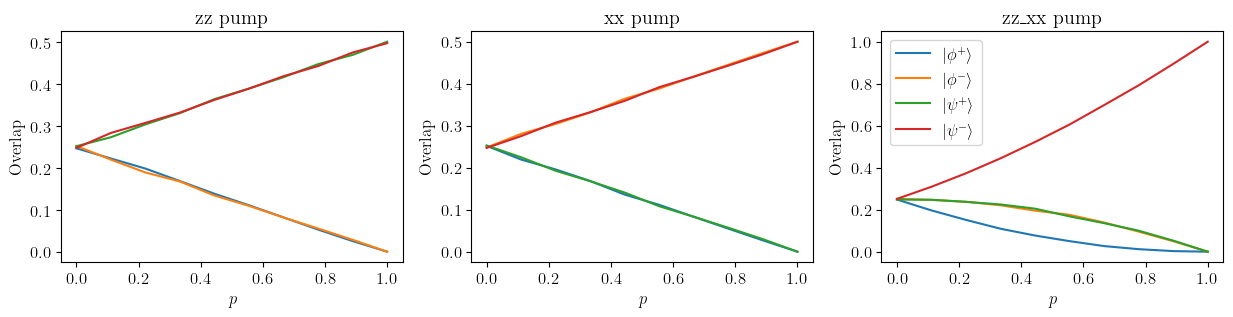
\includegraphics[width=\textwidth]{images/reservoir-engineering-simulation.png}
    \caption{Simulation of a quantum circuit.%
      \label{fig:reservoir-engineering-simulation}}
  \end{figure}


  \subsection{Amplitude Damping}
  We plot the dynamics of the entanglement witness for the amplitude damping channel.

  \begin{figure}
    \centering
    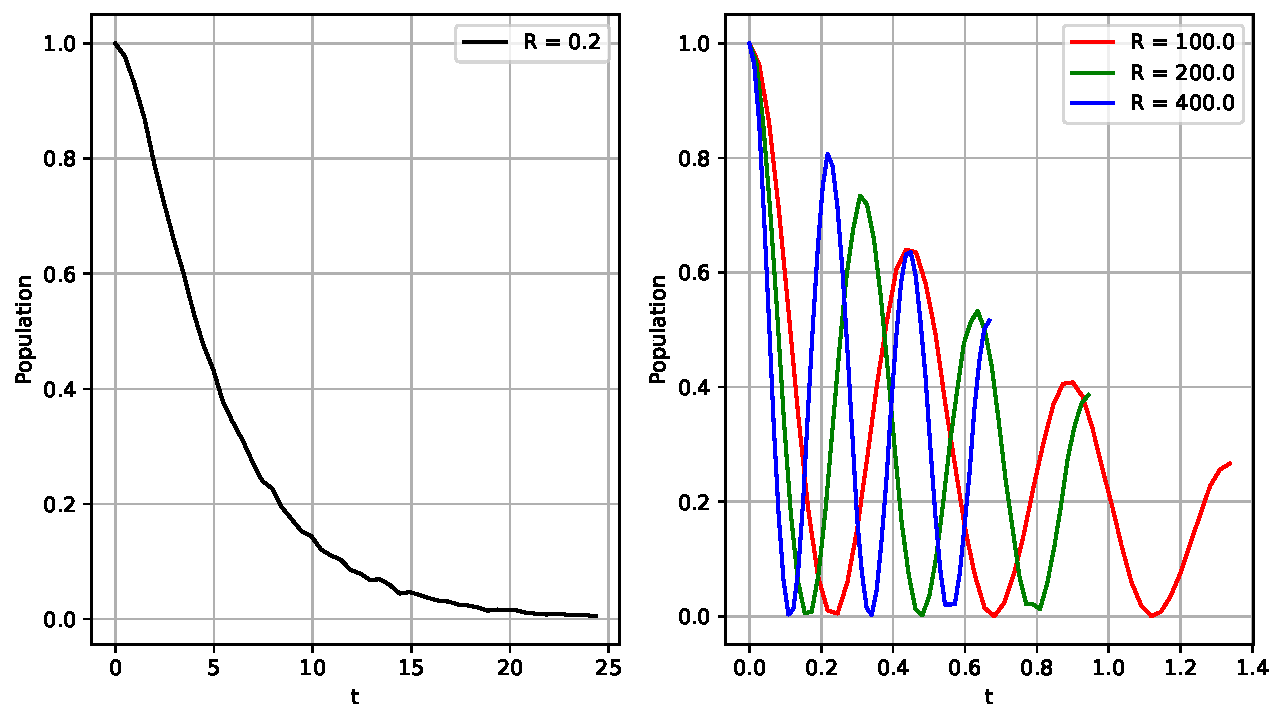
\includegraphics[width=0.7\textwidth]{images/amplitude_damping_population_non_markovianity.pdf}
    \caption{The comparison for damping time for different \( R \).%
      \label{fig:amplitude_damping_population}}
  \end{figure}

  % TODO:
  %  - Where is this supposed to go? Needs reference to specific figure.
  The witness clearly shows oscillatory behaviour and therefore properly signals the presence of memory effects.


  \subsection{Depolarization and Pauli Channels}

  \begin{figure}
    \centering
    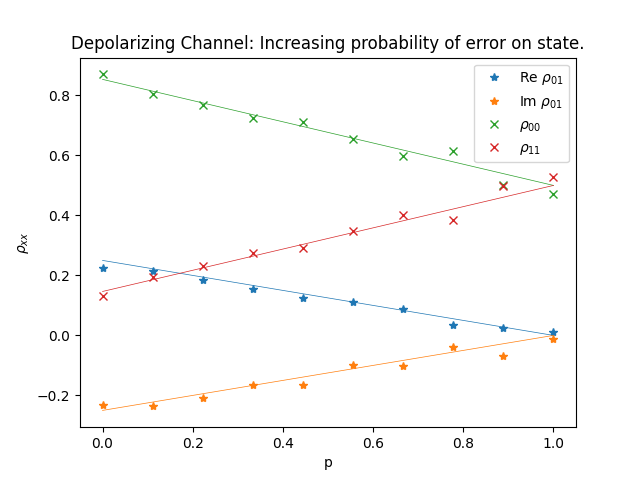
\includegraphics[width=0.7\textwidth]{images/depolarizing_probability_state.png}
    \caption{Increasing probability of error for depolarizing channel on stationary system.%
      \label{fig:depolarizing_probability_state}}
  \end{figure}

  % TODO:
  %  - Manual cropping partially killed legend. Can't see what the colors mean.
  \begin{figure}
    \centering
    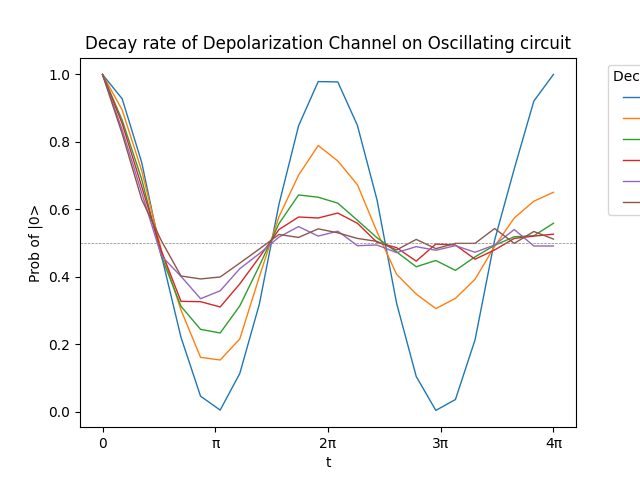
\includegraphics[width=0.7\textwidth]{images/depolarization_decay_oscillating.png}
    \caption{Depolarization channel of increasing decay rate on oscillating channel}
    \label{fig:depolarization_deay_oscillating}
  \end{figure}

  \begin{figure}
    \centering
    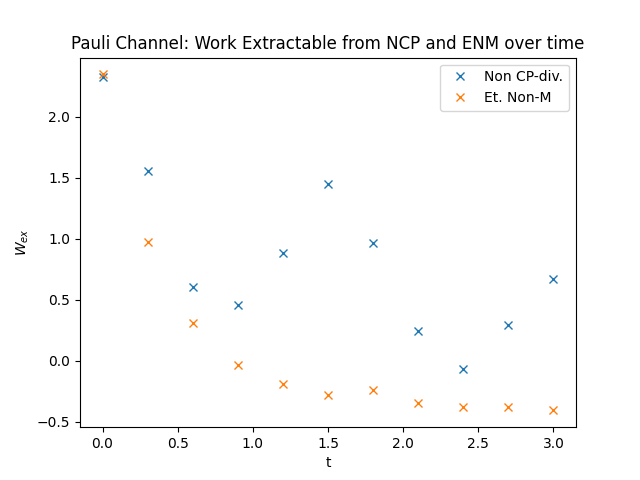
\includegraphics[width=0.7\textwidth]{images/Pauli_work_extractable.png}
    \caption{Work extractable of Pauli channel methods over time.%
      \label{fig:Pauli_work_extractable}}
  \end{figure}

  \printbibliography
\end{document}